\documentclass[conference]{IEEEtran}
\IEEEoverridecommandlockouts
% The preceding line is only needed to identify funding in the first footnote. If that is unneeded, please comment it out.
\usepackage{cite}
\usepackage{amsmath,amssymb,amsfonts}
\usepackage{algorithmic}
\usepackage{graphicx}
\usepackage{textcomp}
\usepackage{xcolor}
\usepackage{mathrsfs}
\def\BibTeX{{\rm B\kern-.05em{\sc i\kern-.025em b}\kern-.08em
    T\kern-.1667em\lower.7ex\hbox{E}\kern-.125emX}}
\begin{document}

\title{EE 565 Machine Learning\\
Project 1 Report\\
\thanks{The author is with the Klipsch School of Electrical and Computer Engineering, New Mexico State University (NMSU), Las Cruces NM 88003 USA. e-mail: tonydero@nmsu.edu}
}

\author{\IEEEauthorblockN{Anthony M. DeRocchis}}

\maketitle

\begin{abstract}

In this report I explore the results of applying various Machine Learning algorithms to randomly generated synthetic data sets. These data sets are to be used in subsequent projects for test and evaluation of algorithm performance. In addition to the randomly generated data sets, I also visualize some predefined data sets by loading the relevant data from files and plotting.

\end{abstract}

\begin{IEEEkeywords}
	Data Sets
\end{IEEEkeywords}

\section{Introduction}

This is a report of my solutions and findings from Project 1. I have created functions implementing the K-Means (batch and online versions), Polynomial Regression, and K-Nearest Neighbors algorithms. Attempts were made to vectorize as much of it as possible to improve performance, however the algorithms are far from optimal in their current states. Additionally, I will discuss the effects of changing various factors in several of the problems on their respective solutions.

\section{Problem 1: Batch $K$-means}
\subsection{Circular Symmetric Gaussians Data Set and $K=2$}
First, I looked at how well the batch version of the $K$-means algorithm was able to recover the true data centers as the centroids while varying the number of training data points from 10 to 500. Figure \ref{fig:p1pa} shows the number of training points versus the error. The error is calculated as the sum of the Euclidean distance from the actual centers to the respective centroid locations estimated using $K$-means.

Next, I looked at how the initialization of the centroids affects the outcome. Instead of randomly initializing the centroids to a set of $K$ training points, I manually initialized them both to (0,0), and then to (100,0) and (0,0). In the former case #TODO, but in the latter case, they did not converge properly, as all points were associated with a single centroid upon convergence.

For the final experiment using $K=2$, I considered a data set consisting of 50 data points, and looked at how many iterations it took to converge, on average. The mean value was approximately $3.76$, with a minimum of $2$ iterations, and a maximum of $7$ iterations.

\subsection{Circular Symmetric Gaussians Data Set and $K\geq2$}
Again using a set of 50 data points, I examined what happens to the cost function $J$ as $K$ took on values in the range of 2 to 20. Figure \ref{fig:p1pd} shows that as $K$ increased, $J$ decreased.

Then I examined the effect of three various initializations on a data set of 50 points with $K=5$. Figure \ref{fig:p1pe} shows that unless the centroids were initialized very poorly, two of the five at least converged in the right direction, with the orange "x" representing the initialization points, and the red "+" representing the location of the centroids upon convergence.

\section{Problem 2: Online $K$-means}
\subsection{Circular Symmetric Gaussians Data Set and $K=2$}
Next, I examined the effect of varying the learning rate, $\eta$, on the number of epoch iterations. Figure \ref{fig:p2pa} shows that smaller values of $\eta$ result in fewer epoch iterations until convergence.

\section{Problem 3: $K$-means Application: Image Segmentation}
\section{Problem 4: Polynomial Curve Fitting}
\subsection{Model Selection}
\subsection{Training Data Size}
\section{Problem 5: Polynomial Regression with Regularization}
\section{Problem 6: $K$-Nearest Neighbors Classification}
\subsection{Concentric Gaussians Data Set}
\subsection{Double Moon Data Set}
\subsection{Gaussian XOR Data Set}

A function named "circGauss" was written which returns $N$ samples drawn from a circular symmetric multi-variate Gaussian distribution of dimension $D$ with variance $\sigma^2$

\begin{align}
	X \thicksim
	\begin{bmatrix}
		\mathcal{N}($\mu_1$, $\sigma^2$) \\
		\mathcal{N}($\mu_2$, $\sigma^2$) \\
		\vdots \\
		\mathcal{N}($\mu_D$, $\sigma^2$)
        \end{bmatrix}
\end{align}

where $\mu_k$ is the mean for the $k$th dimension \cite{b1}. The function was used to generate a data set (shown in figure \ref{fig:circgauss}) consisting of samples drawn from two circular symmetric multi-variate Gaussian distributions in two dimensions with one distribution at the origin and one at the point $(5, 5)$, where both distributions have $\sigma^2 = 3$.

\section{Problem 2: Double Moon Data Set}
A function named "doublemoon" was written which returns $N$ samples drawn from a double moon distribution \cite{b2}. Figure \ref{fig:doublemoon} shows an example of data drawn from the double moon distribution with parameters $N=500$ samples, $d=0$, $r=1$, and $w=0.6$. In figure \ref{fig:doublemoon} the members of class $\mathscr{C}_1$ are plotted as "blue +" and $\mathscr{C}_2$ are plotted as "green x".

\section{Problem 3: Concentric Gaussian Data Set}
A function named "concentGauss" was written which returns $N$ samples drawn from a data set consisting of a circular symmetric Gaussian centered at the origin with variance $\sigma^2_{center}$ and a Gaussian annulus centered at the origin with radius mean $r$ and variance $\sigma^2_{outer}$. Figure \ref{fig:concentgauss} shows an example of data drawn from the concentric Gaussian data set with $N=500$ samples, $\sigma^2_{center}=1$, $r=5$, and $\sigma^2_{outer}=1$ with members of class $\mathscr{C}_1$ plotted as "blue +" and class $\mathscr{C}_2$ plotted as "green x". 

\section{Problem 4: Gaussian XOR Data Set}
A function named "gaussX" was written which returns $N$ samples drawn from a Gaussian XOR distribution. Figure \ref{fig:gaussx} shows an example of data drawn from a Gaussian XOR data set with $N=500$ samples and $\sigma^2=1$, where members of class $\mathscr{C}_1$ are plotted as "blue +" and members of $\mathscr{C}_2$ as "green x".

\section{Problem 5: Noisy Sinusoidal Data Set}
\subsection{Randomly Generated}\label{section:randomgen}
A function named "noisySin" was written which returns $N$ samples drawn from a noisy sine distribution with a sinusoidal amplitude of $1$ and period $2\pi$, where the added noise has a variance $\sigma^2$. Figure \ref{fig:noisysingen} shows an example of data drawn from a noisy sine data set with $N=50$ samples and $\sigma^2=0.05$, where the noise-added sinusoidal data is plotted as "blue o" and the clean sinusoidal waveform is plotted as a green curve.

\subsection{Loading from File}
To demonstrate the instance of needing to use a pre-existing, given, data set, the file "curvefitting.txt" was loaded. The data set consists of input $x$ and target $t$ values. These values were plotted, as shown in figure \ref{fig:noisysinfile}, using the same method as section \ref{section:randomgen}, with the noise-added sinusoidal data plotted as "blue o", and the clean sinusoid plotted as a green curve.

\section{Problem 6: Old Faithful Data Set}
The Old Faithful data set was loaded from the file "faithful.txt" and plotted. The results are shown in figure \ref{fig:oldfaithful}.

\section{Problem 7: Neural Spike Data Set}
The Neural Spike data set was loaded from the file "spikes.csv" and plotted. The results are shown in figure \ref{fig:neuralspikes}.

\section{Conclusion}
In this project I loaded, generated, and visualized several data sets which will be useful for test and evaluation of machine learning algorithms. In addition, this document serves as a simple example of what is expected in a project write-up.


\begin{thebibliography}{00}
\bibitem{b1} C. Bishop, Pattern Recognition and Machine Learning. Springer, 2006.
\bibitem{b2} S. Haykin, Neural Networks and Learning Machines. Prentice Hall, 2009.
\end{thebibliography}

\begin{figure}[p!]
\centerline{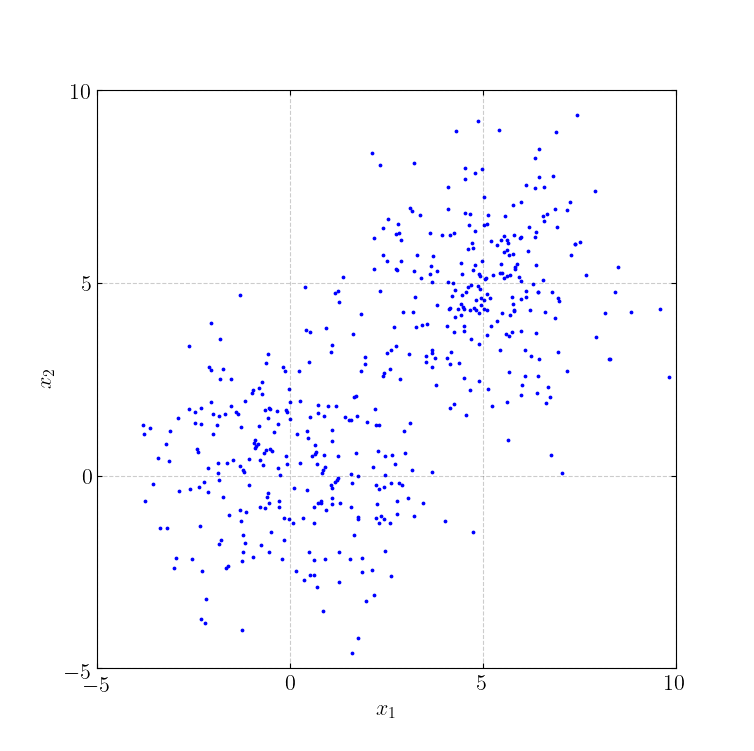
\includegraphics[trim=0 0 0 0, clip, width=\columnwidth]{Figure_1.png}}
\caption{A data set consisting of samples drawn from two circular symmetric multi-variate Gaussian distributions with paramters $\sigma^2=3$ and $\mu=(0,0)$ for one and $\mu=(5,5)$ for the other.}
\label{fig:circgauss}
\end{figure}

\begin{figure}[p!]
\centerline{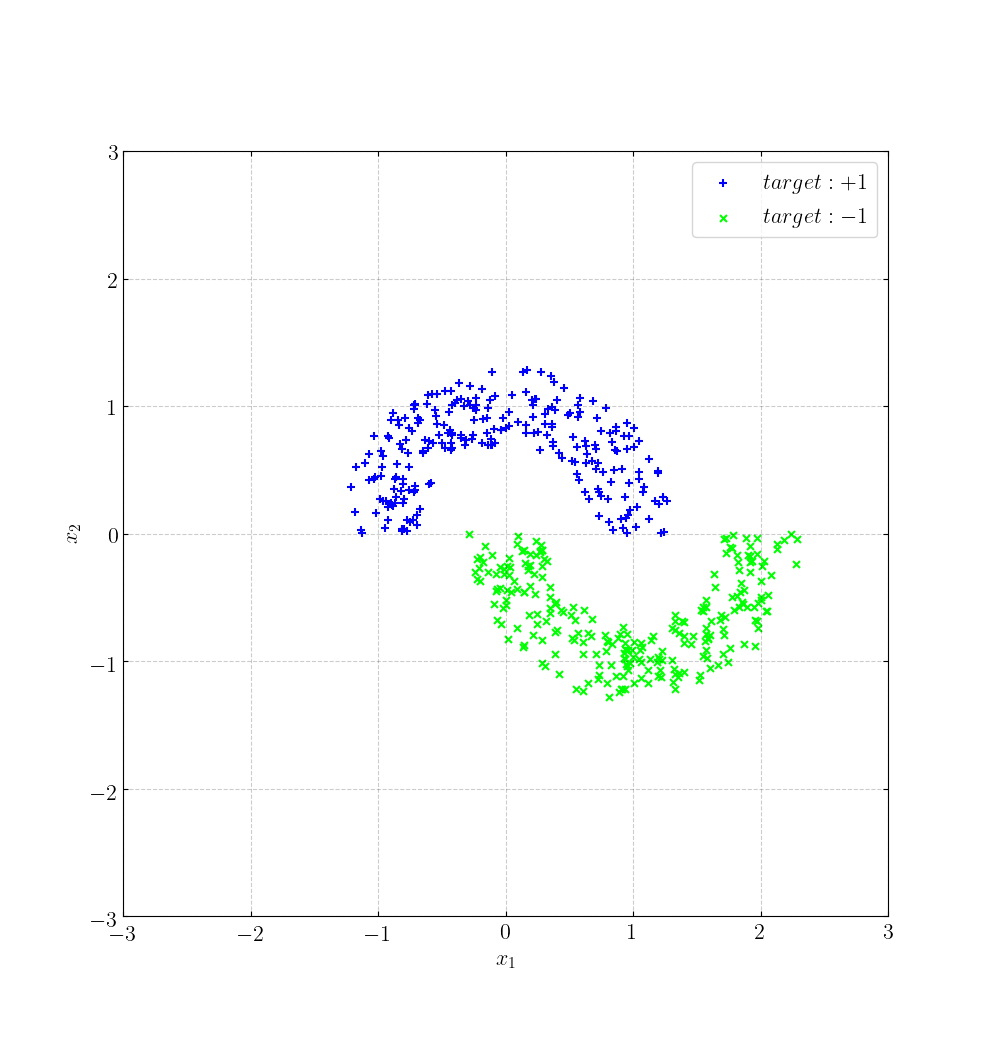
\includegraphics[trim=0 0 0 0, clip, width=\columnwidth]{Figure_2.png}}
\caption{A data set consisting of samples drawn from a double moon distribution with parameters $N=500$ samples, $d=0$, $r=1$, and $w=0.6$. The members of class $\mathscr{C}_1$ are plotted as "blue +" and $\mathscr{C}_2$ as "green x". }
\label{fig:doublemoon}
\end{figure}

\clearpage

\begin{figure}[p!]
\centerline{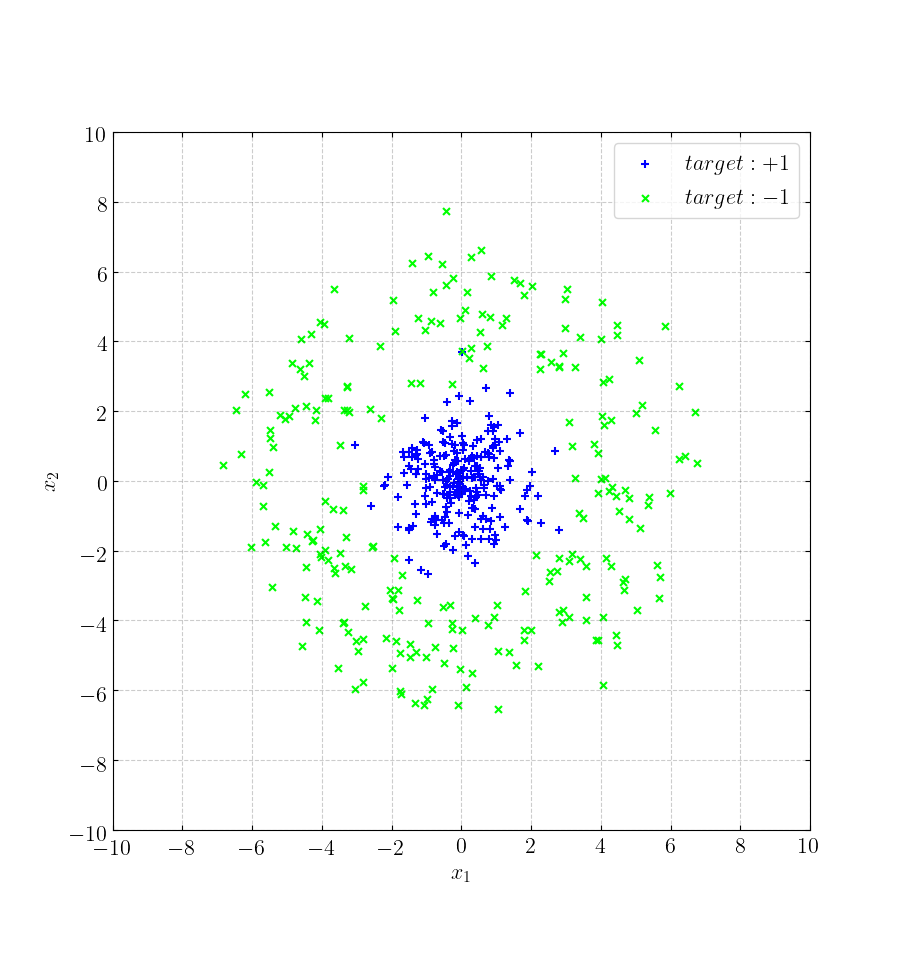
\includegraphics[trim=0 0 0 0, clip, width=\columnwidth]{Figure_3.png}}
\caption{A data set consisting of samples drawn from a circular symmetric Gaussian centered at the origin with variance $\sigma^2_{center}$ and a Gaussian annulus centered at the origin with radius mean $r$ and variance $\sigma^2_{outer}$ with parameters $N=500$ samples, $\sigma^2_{center}=1$, $r=5$, and $\sigma^2_{outer}=1$. Members of class $\mathscr{C}_1$ are plotted as "blue +" and class $\mathscr{C}_2$ plotted as "green x".}
\label{fig:concentgauss}
\end{figure}

\begin{figure}[p!]
\centerline{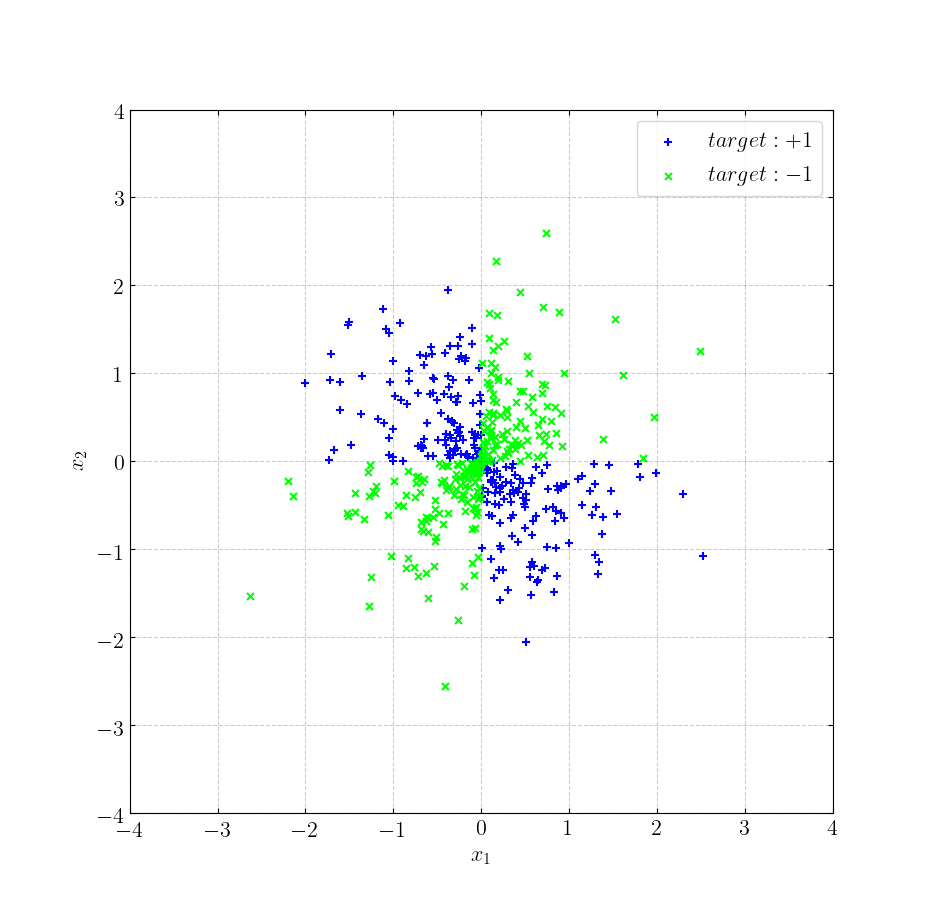
\includegraphics[trim=0 0 0 0, clip, width=\columnwidth]{Figure_4.png}}
\caption{A data set consisting of samples drawn from a Gaussian XOR distribution with parameters $N=500$ samples and $\sigma^2=1$. Members of class $\mathscr{C}_1$ are plotted as "blue +" and members of $\mathscr{C}_2$ as "green x".
}
\label{fig:gaussx}
\end{figure}

\begin{figure}[p!]
\centerline{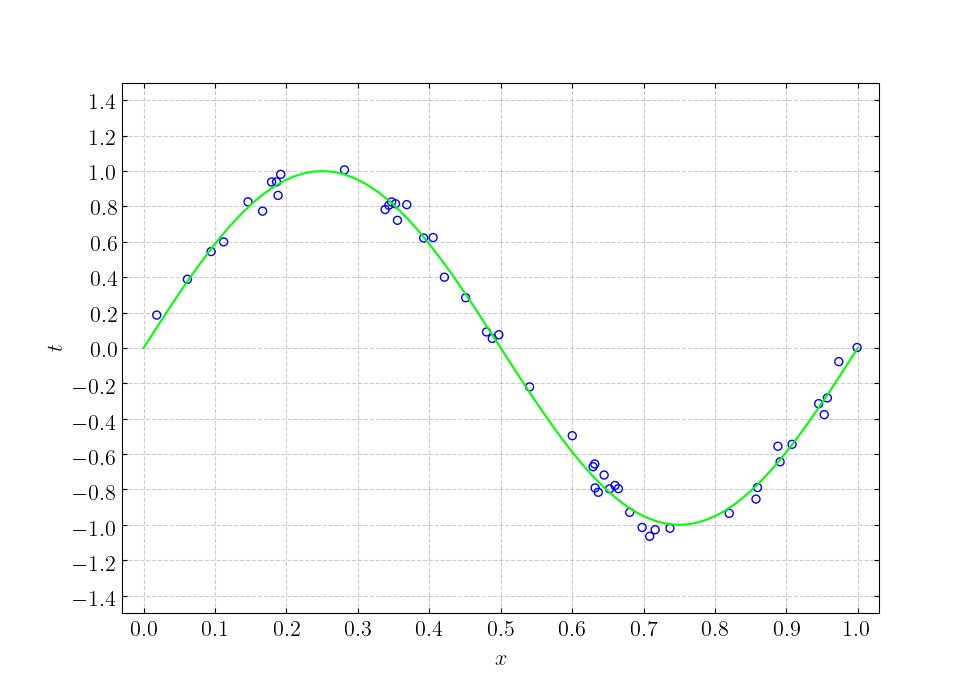
\includegraphics[trim=0 0 0 0, clip, width=\columnwidth]{Figure_5.png}}
\caption{A data set consisting of samples drawn from a noisy sine distribution with a sinusoidal amplitude of $1$ and period $2\pi$, where the added noise has a variance $\sigma^2$ with parameters $N=50$ samples and $\sigma^2=0.05$. The noise-added sinusoidal data is plotted as "blue o" and the clean sinusoidal waveform is plotted as a green curve.}
\label{fig:noisysingen}
\end{figure}

\begin{figure}[p!]
\centerline{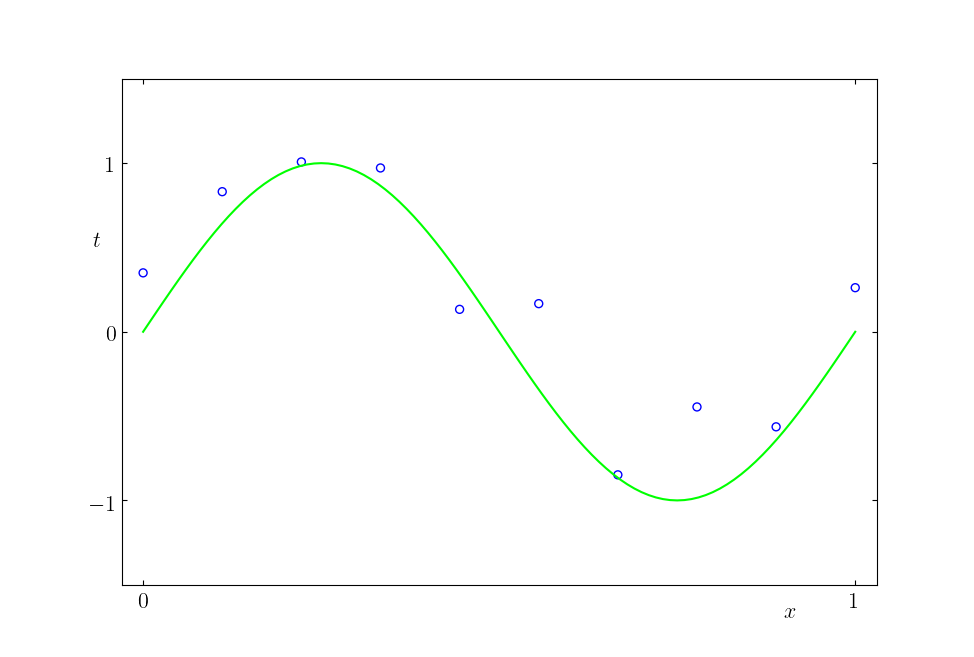
\includegraphics[trim=20 0 40 0, clip, width=\columnwidth]{Figure_6.png}}
\caption{The data set read from the file "curvefitting.txt" plotted as "blue o" on top of a clean sinusoidal waveform plotted as a green curve.}
\label{fig:noisysinfile}
\end{figure}

\begin{figure*}[p!]
\centerline{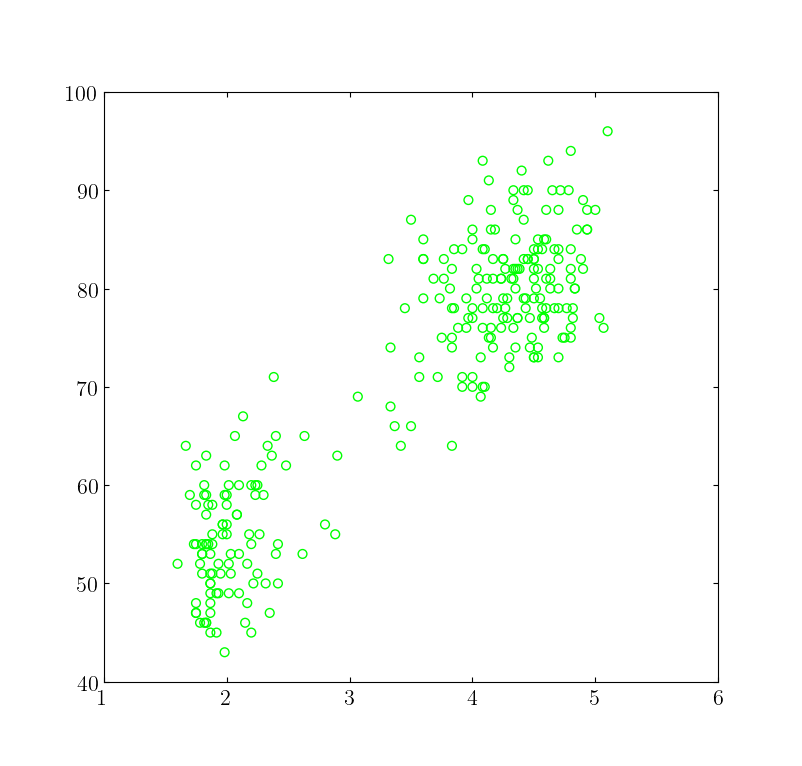
\includegraphics[trim=0 0 0 0, clip, width=300]{Figure_7.png}}
\caption{The data set read from the file "faithful.txt" and plotted.}
\label{fig:oldfaithful}
\end{figure*}

\begin{figure*}[p!]
\centerline{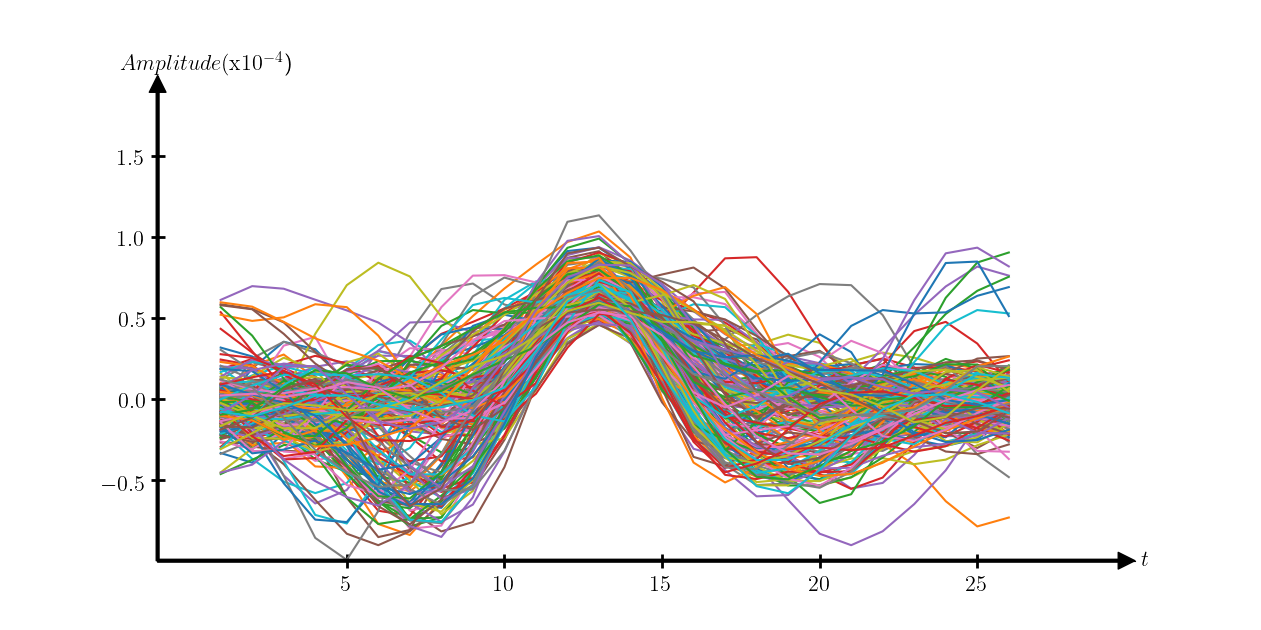
\includegraphics[trim=30 0 30 0, clip, width=360]{Figure_8.png}}
\caption{The data set read from the file "spikes.csv", with the amplitudes scaled up by a factor of $10^4$ and plotted.}
\label{fig:neuralspikes}
\end{figure*}

\end{document}
